\documentclass[11pt,a4paper]{article}

% --- packages ---
\usepackage[margin=1in]{geometry}
\usepackage{times}
\usepackage{amsmath,amssymb}
\usepackage{booktabs}
\usepackage{graphicx}
\usepackage{xcolor}
\usepackage{hyperref}
\usepackage{natbib}
\usepackage{tikz}
\usetikzlibrary{arrows.meta,positioning,fit,calc}
\usepackage{microtype}
\usepackage[T1]{fontenc}
\usepackage[utf8]{inputenc}

\hypersetup{
  colorlinks=true,
  linkcolor=blue!50!black,
  citecolor=blue!50!black,
  urlcolor=blue!40!black
}

% Honesty macros
\newcommand{\established}{\textcolor{green!40!black}{\textsc{[Established]}}}
\newcommand{\hypothesis}{\textcolor{orange!70!black}{\textsc{[Hypothesis]}}}
\newcommand{\provisional}{\textcolor{purple!60!black}{\textsc{[Provisional]}}}

\title{\textbf{RQL: A Portable Intermediate Representation\\
for Retrieval Plans in RAG Systems}\\[0.4em]
\large Incremental research draft --- not a camera-ready submission}
\author{Vijay Kumar\\
\textit{Research draft, Europe/Dublin}\\
\texttt{vijaykumarjob0701/rql-rag-query-language}}
\date{16 September 2026}

\begin{document}
\maketitle

\begin{center}
\small
\textbf{Draft status.} Structured for growth into a citable article/thesis.
Claims are labelled \established{}, \hypothesis{}, or \provisional{}.
No fabricated experimental results. Not claimed ready for NeurIPS, VLDB, or arXiv acceptance.
\end{center}

\begin{abstract}
Retrieval-augmented generation (RAG) systems compose embedding search, lexical retrieval, metadata and ACL filters, hybrid fusion, reranking, and sometimes graph or multi-hop expansion.
Today those stages are usually glued together in application code against vendor-specific vector-database APIs.
This draft proposes \textbf{RQL (Retrieval Query Language)} not merely as ``SQL for vectors'', but as a \textbf{portable intermediate representation for retrieval plans}: a small algebra over scored evidence, plus cost-based physical planning under recall, latency, and ACL constraints, compiling through adapters to heterogeneous backends.

We separate \established{} survey material from \hypothesis{} original design and from \provisional{} literature pending multimodal re-read.
A careful multimodal pass over ACORN~\citep{patel2024acorn} grounds filtered-ANN physical strategies.
We define an evaluation \emph{plan} and reproducibility layout; we do \textbf{not} report unreproduced benchmark scores.
\end{abstract}

\section{Introduction}
\label{sec:intro}

\subsection{Motivation}
Modern RAG stacks must retrieve \emph{evidence}---chunks, passages, entities, paths---under mixed modalities: dense vectors, sparse/BM25 channels, structured predicates (including ACLs), and increasingly late-interaction or graph expansion~\citep{lewis2020rag} \established{}.
Vector databases expose powerful but \textbf{non-portable} interfaces (JSON filters, GraphQL operators, SQL extensions, Redis commands, Cypher search).
As a result, three operational properties leave the plan and hide in glue code:

\begin{description}[leftmargin=1.6cm,style=nextline]
  \item[Accuracy.] Hybrid fusion (e.g.\ reciprocal rank fusion~\citep{cormack2009rrf}), over-fetch+rerank, and multi-query rewriting improve recall only when stages are explicit and tunable \established{} as IR practice; RQL makes them plan nodes \hypothesis{}.
  \item[Latency.] Filter placement (pre vs.\ post vs.\ subgraph vs.\ specialised label graphs vs.\ iterator ANN) and ANN parameters dominate end-to-end cost~\citep{patel2024acorn,gollapudi2023filtered,zhang2023vbase,lin2025fanns} \established{}.
  \item[Reliability.] Silent empty results, client-side ACL filtering, and irreproducible \texttt{efSearch} folklore are operational failures; plans with \texttt{EXPLAIN} and mandatory predicate pushdown targets are the proposed remedy \hypothesis{}.
\end{description}

\subsection{Idea in one paragraph}
\textbf{RQL is a portable IR for retrieval plans}---an algebra over scored multisets of evidence together with a Cascades/Calcite-inspired physical planner that chooses filtered-ANN and fusion strategies under explicit recall/latency/ACL contracts, then compiles via polystore-like shims to concrete engines~\citep{begoli2018calcite,substrait,duggan2015bigdawg} \hypothesis{} (adjacency; not an embedding of those systems).
The textual DSL is a frontend, not the contribution's centre of mass.

\subsection{Contributions}
\label{sec:contributions}
\begin{enumerate}[leftmargin=*]
  \item \textbf{Problem formulation} for portable, ACL-safe, budget-aware retrieval plans (Section~\ref{sec:problem}).
  \item \textbf{Hypothesized retrieval algebra and physical operator set} that packages established mechanisms (RRF, Condorcet, linear/CC, MaxSim, PLAID/MUVERA, HyDE, MMR, FANNS FilterExec modes, BlinkDB-inspired budgets) as one IR (Sections~\ref{sec:algebra}--\ref{sec:optimizer}) \hypothesis{}; prior mechanisms labelled \established{} / \authoronly{} where appropriate.
  \item \textbf{Compilation doctrine + offline prototype:} docs-only vendor matrix (journal 0020), LogicalPlan/PhysicalPlan JSON Schema freeze \texttt{0.1.0-draft} (journal 0021), toy parser / planner / emit / E2E CLI (journals 0022--0024, 0026) with 12/12 schema-validated toy runs (Section~\ref{sec:compilation}) \hypothesis{}.
  \item \textbf{Related-work positioning} with multimodal re-reads of ACORN, VBASE, Filtered-DiskANN, FANNS survey, RRF/Condorcet/Bruch/Chen, ColBERT/PLAID/MUVERA, HyDE, MMR, BlinkDB, and Substrait/Calcite adjacency (Section~\ref{sec:related}).
  \item \textbf{Honest evaluation split:} unit/E2E/plumbing measurements vs remaining P0 (SIFT1M), P1 (live adapters), and judgment-bearing RAG work (Section~\ref{sec:eval})---no fabricated metrics.
\end{enumerate}

\subsection{Reader's guide: how to implement / run RQL today}
\label{sec:readers-guide}
If you are an engineer who wants to \emph{touch} the stack before reading the algebra:

\begin{enumerate}[leftmargin=*]
  \item \textbf{Skim the idea:} this section + Figure~\ref{fig:e2e-pipeline} (end-to-end offline pipeline) and Figure~\ref{fig:stack} (plan layers).
  \item \textbf{Hello RQL (offline, no vector DB):}
  \begin{verbatim}
cd experiments/harness
python rql_pipeline.py \
  --rql ../../examples/toy/01-hybrid-rrf.rql \
  --profile qdrant --validate \
  --out ../../experiments/results/e2e/my_run
  \end{verbatim}
  Expect LogicalPlan JSON, PhysicalPlan JSON, and a vendor request \emph{sketch} marked \texttt{notExecuted}.
  Full toy matrix: four queries $\times$ three profiles $= 12/12$ (see \texttt{experiments/results/e2e/run\_validate.txt}).
  \item \textbf{Schemas:} \texttt{schemas/logical-plan.schema.json}, \texttt{schemas/physical-plan.schema.json} (\texttt{0.1.0-draft}).
  \item \textbf{What is \emph{not} ready:} live Qdrant/ES/pgvector smoke, SIFT1M FANNS P0, BEIR/RAG with judgments---see Section~\ref{sec:eval} and \texttt{experiments/HUMAN\_TODOS.md}.
\end{enumerate}
More detail and file paths appear in Section~\ref{sec:hello-rql}.

\subsection{Paper roadmap}
Section~\ref{sec:background} recalls ANN, hybrid fusion, late interaction, and RAG stages.
Section~\ref{sec:related} positions RQL against vector-DB APIs, FANNS, fusion, late interaction, IR languages, and portable-plan systems.
Section~\ref{sec:problem} states requirements and non-goals.
Sections~\ref{sec:algebra}--\ref{sec:optimizer} present the algebra and physical planning (plain language first, then formalism).
Section~\ref{sec:compilation} covers adapters, schemas, and the offline prototype.
Section~\ref{sec:apps} maps common RAG patterns to example \texttt{.rql} files.
Section~\ref{sec:eval} separates measured plumbing from citation-grade remaining work.
Section~\ref{sec:threats} lists limitations; Section~\ref{sec:conclusion} gives actionable next steps.
Appendix~\ref{sec:repro} is the reproducibility checklist.

\section{Background}
\label{sec:background}

\subsection{Approximate nearest neighbour search}
Graph indices such as HNSW~\citep{malkov2018hnsw} and disk-oriented graphs (DiskANN line) underpin production vector search.
Search quality/latency is controlled by parameters (e.g.\ candidate list size), yielding recall--throughput curves rather than exact SQL cardinalities \established{}.

\subsection{Hybrid vector + predicate search}
Applications need ANN jointly with structured predicates.
Common strategies include \textbf{pre-filtering}, \textbf{post-filtering}, specialised low-cardinality equality indices, and \textbf{predicate-subgraph} traversal as in ACORN~\citep{patel2024acorn} \established{} (see Section~\ref{sec:related}).

\subsection{Hybrid lexical--dense fusion}
Reciprocal Rank Fusion (RRF) combines ranked lists without score calibration~\citep{cormack2009rrf} \established{}.
Production engines also expose weighted linear fusion and learned rankers; choice is workload-dependent \provisional{}.

\subsection{Late interaction}
ColBERT-style late interaction~\citep{khattab2020colbert} and subsequent engines/rewrites (e.g.\ MUVERA~\citep{jayaram2024muvera}) show that multi-vector retrieval admits planner rewrites \provisional{} (pending dedicated multimodal reads).

\subsection{RAG as a staged pipeline}
A typical RAG retrieve path is: embed $\rightarrow$ search channels $\rightarrow$ filter $\rightarrow$ fuse $\rightarrow$ (rerank) $\rightarrow$ expand/traverse $\rightarrow$ generate.
RQL aims to name these stages as plan operators rather than ad-hoc functions \hypothesis{}.

\section{Related work}
\label{sec:related}

\subsection{Vector database interfaces}
Commercial and OSS systems expose vendor-specific query surfaces (metadata filters, hybrid search APIs, SQL extensions such as pgvector).
Survey details and URLs live in the companion research package; none is a cross-vendor ANSI-SQL analogue for multi-stage RAG plans \established{} (landscape notes).

\subsection{Filtered ANN / FANNS}
\paragraph{Lin et al.\ survey (multimodal re-read).}
Lin et al.~\citep{lin2025fanns} formalise hybrid datasets/queries and propose a pruning-focused taxonomy---\textbf{VSP}, \textbf{VJP}, \textbf{SJP}, \textbf{SSP}---classifying 17 algorithm families (A1--A17; Figs.~1--2).
They further argue that hybrid query difficulty depends on \emph{selectivity and distribution} (ID/POD/OOD; Figs.~3--6), and highlight combining multiple FANNS algorithms with dynamic selection as a system-level direction (\S6.3).
Pass~1--5 notes (journal 0019; \texttt{knowledge/reads/fanns-lin2025-2505.06501/}) treat the \textbf{taxonomy and A1--A17 map} as \established{} survey structure grounding $\mathrm{FilterExec}$ packaging; author Fig.~3 recall curves remain unreproduced \provisional{}.

\paragraph{ACORN (multimodal re-read).}
Patel et al.~\citep{patel2024acorn} argue that pre- and post-filtering are brittle under selectivity and query--predicate correlation, and that specialised equality indices constrain predicate cardinality.
They propose denser, predicate-agnostic HNSW variants (ACORN-$\gamma$, ACORN-1) that \emph{search the predicate subgraph} to approximate an oracle HNSW over surviving vectors.
Our Pass~1--5 notes (journal 0006; OKF bundle under \texttt{knowledge/reads/acorn-2403.04871/}) treat author QPS claims as \textbf{not reproduced here} \established{} for the problem taxonomy; \provisional{} for unreproduced numeric speedups.

\paragraph{Filtered-DiskANN (multimodal re-read).}
Gollapudi et al.~\citep{gollapudi2023filtered} change \emph{graph construction} (FilteredVamana / StitchedVamana) so edges respect geometry and labels, then search with label-aware greedy expansion.
Pass~1--5 notes (journal 0010; \texttt{knowledge/reads/filtered-diskann-www23/}) ground $\mathrm{FilterExec}=\mathrm{SPECIALIZED}$ for equality/label predicates; complex SQL-like filters remain an author-stated open problem \established{} for the specialised-graph idea; \provisional{} for unreproduced QPS curves.

\paragraph{VBASE (multimodal re-read).}
Zhang et al.~\citep{zhang2023vbase} formalise \emph{relaxed monotonicity} and expose ANN traversal as Volcano $\mathrm{Open}/\mathrm{Next}/\mathrm{Close}$ inside PostgreSQL, enabling filter-during-traversal, multi-column TopK, range filters, and vector joins without a predicted over-fetch $K'$.
Pass~1--5 notes (journal 0009; \texttt{knowledge/reads/vbase-osdi23/}) ground $\mathrm{FilterExec}=\mathrm{ITERATIVE}$ and a concrete path for $\mathrm{VSimJoin}$ \established{} for the iterator architecture; \provisional{} for unreproduced latency claims.

\subsection{Rank fusion (RRF and linear/CC)}
\paragraph{Cormack et al.\ (multimodal re-read).}
Cormack, Clarke, and B\"{u}ttcher~\citep{cormack2009rrf} define Reciprocal Rank Fusion as
\(\mathrm{RRFscore}(d)=\sum_{r\in R} 1/(k+r(d))\) with \(k=60\) fixed after a pilot study.
RRF is unsupervised and \emph{rank-only} (no requirement that channel scores be calibrated), unlike CombMNZ.
Pass~1--5 notes (journal 0011; \texttt{knowledge/reads/rrf-cormack-sigir09/}) treat the \textbf{formula and default \(k\)} as \established{} IR prior art for logical \(\mathrm{Fuse}_{rrf}\); author TREC/LETOR MAP tables are \textbf{not reproduced here} \provisional{} as unreproduced empirics.

Montague and Aslam~\citep{montague2002condorcet} introduce \emph{Condorcet-fuse}: a majoritarian (Social Choice) fusion that sorts the candidate pool using a pairwise majority runoff over input rankings as the comparison function (\(O(nk\log n)\); ranks only).
Their Fig.~1 taxonomy places Condorcet-fuse beside Borda-fuse/rCombMNZ in the ranks-only / no-training cell, opposite CombMNZ on the score axis; weighted Condorcet and dependence filtering (correlated-run prune) are optional variants.
Pass~1--5 notes (journal 0018; \texttt{knowledge/reads/montague-aslam-cikm02-condorcet/}) treat the \textbf{pairwise-majority sort mechanism and Fig.~1 fusion-input taxonomy} as \established{} literature for logical \(\mathrm{Fuse}_{condorcet}\) as a Fuse-family sibling of \(\mathrm{Fuse}_{rrf}\); author TREC MAP / sign-test tables remain \provisional{} / AUTHOR-only.
Cormack et al.\ later report RRF matching or beating Condorcet Fuse on their suites \established{} as an AUTHOR comparison (journal 0011) --- motivating RRF as the portable default while retaining Condorcet as an optional majoritarian sibling \hypothesis{}.

\paragraph{Bruch et al.\ (multimodal re-read).}
Bruch, Gai, and Ingber~\citep{bruch2023fusion} analyse hybrid lexical--semantic fusion via a \emph{convex combination} of normalised channel scores (TM2C2: theoretical min--max + \(\alpha\)) versus RRF (including parametric \(\eta_{\mathrm{Lex}},\eta_{\mathrm{Sem}}\) and RRF-CC).
They argue CC learning is largely agnostic among monotone normalisers, RRF is parameter-sensitive, and CC is sample-efficient; on their suite they report TM2C2 beating default RRF on NDCG (disagreement with Chen et al.).
Pass~1--5 notes (journal 0016; \texttt{knowledge/reads/bruch-arxiv-2210.11934/}) treat the \textbf{CC/TM2C2 formulas, normalisation role, and RRF-vs-CC delineation} as \established{} literature mechanisms for logical \(\mathrm{Fuse}_{linear}\) (with \(\mathrm{Fuse}_{ltr}\) as the learned multi-parameter end of the continuum); author Recall/NDCG tables remain \provisional{} / AUTHOR-only.

\paragraph{Chen et al.\ (cite-chase from Bruch [5]; multimodal re-read).}
Chen, Zhang, Lu, Bendersky, and Najork~\citep{chen2022ood} study \emph{zero-shot} hybrid retrieval and fuse lexical (+expansion) with deep (NPR) channels via RRF (\(k{=}60\)).
They argue score linear interpolation needs min--max normalisation and \(\alpha\) tuning that conflicts with zero-shot transfer; on Robust04 and TREC-COVID, their best-tuned min--max BM25$+$NPR interpolation still underperforms RRF(BM25, NPR) by about 3\% relative Recall@1K (Fig.~2; primary metric Recall@1K/MAP, not NDCG).
Pass~1--5 notes (journal 0017; \texttt{knowledge/reads/chen-ecir2022-2201.10582/}) treat the \textbf{RRF-for-zero-shot mechanism and the linear-interp critique} as \established{} literature; author Recall/MAP tables remain \provisional{} / AUTHOR-only.

\paragraph{Resolving Chen$\leftrightarrow$Bruch (setup disagreement).}
The author-level disagreement is \established{} as a \emph{literature conflict of setups}, not a single false claim: different metrics (Recall@1K vs NDCG), different linear forms (simple min--max \(\alpha\)-interp vs TM2C2 \(\phi_{\mathrm{tmm}}\)), different objectives (zero-shot / no labels vs sample-efficient \(\alpha\) with labels), and different channel/dataset suites.
RQL packaging and the planner preference rule among \(\{\mathrm{Fuse}_{rrf},\mathrm{Fuse}_{linear},\mathrm{Fuse}_{ltr}\}\) remain \hypothesis{} (see \S\ref{sec:fuse-preference}).

\subsection{Late interaction / multi-vector retrieval}
\paragraph{ColBERT (multimodal re-read).}
Khattab and Zaharia~\citep{khattab2020colbert} introduce contextualized late interaction: bags of BERT embeddings scored by MaxSim-sum (Eq.~(3)).
Pass~1--5 notes (journal 0012; \texttt{knowledge/reads/colbert-sigir20/}) treat the \textbf{MaxSim scoring definition and offline document-bag pattern} as \established{}; author MS~MARCO MRR/latency tables are \textbf{not reproduced here} \provisional{}.

\paragraph{PLAID (multimodal re-read).}
Santhanam et al.~\citep{santhanam2022plaid} accelerate ColBERTv2 late-interaction search with a four-stage funnel: centroid-based candidate generation, \emph{centroid interaction} (approximate MaxSim over bags of centroid IDs using $S_{c,q}=CQ^{\top}$), \emph{centroid pruning} by threshold $t_{cs}$, then residual decompression and exact MaxSim.
Pass~1--5 notes (journal 0014; \texttt{knowledge/reads/plaid-cikm22/}) treat the \textbf{centroid-interaction / pruning pipeline (Fig.~5; Eqs.~(2)--(5))} as \established{} literature mechanisms; author GPU/CPU speedup and MRR tables are \textbf{not reproduced here} \provisional{}.

\paragraph{MUVERA (multimodal re-read).}
Dhulipala et al.~\citep{jayaram2024muvera} reduce Chamfer/MaxSim multi-vector search to single-vector MIPS via Fixed Dimensional Encodings, then Chamfer rerank---contrasting PLAID's multi-stage residual-preserving centroid pipeline~\citep{santhanam2022plaid}.
Pass~1--5 notes (journal 0013; \texttt{knowledge/reads/muvera-2405.19504/}) treat the \textbf{FDE reduction + MIPS + MaxSim rerank mechanism} as \established{} literature; RQL rewrite packaging and unreproduced BEIR/PLAID latency numbers remain \hypothesis{} / \provisional{}.

\subsection{IR query languages}
Classical IR languages (Indri, Galago, CQL/SRU) treat ranking as an operator algebra~\citep{metzler2004indri} \provisional{} (URL-verified references; deep re-read pending).
RQL steals composability, not surface syntax fidelity \hypothesis{}.

\subsection{Optimisers, portable plans, polystores}
Apache Calcite~\citep{begoli2018calcite} and Substrait~\citep{substrait} motivate logical/physical separation and portable plan IR.
BigDAWG-style polystores~\citep{duggan2015bigdawg} motivate islands + shims \provisional{}.
BlinkDB~\citep{agarwal2013blinkdb} motivates explicit approximate budgets \provisional{}.

\subsection{Knowledge packaging (methodology, not runtime)}
Google's Open Knowledge Format (OKF) packages knowledge as markdown concepts with YAML frontmatter and graph-shaped links~\citep{okf2025}.
We use OKF-\emph{shaped} bundles for research notes.
We do \textbf{not} claim OKF is part of the RQL execution runtime \established{}.

\subsection{What RQL is not}
RQL is not ``another vendor filter DSL'', not a guarantee of identical recall across HNSW libraries, and not a claim that SQL alone solves multi-stage RAG \hypothesis{}.

\section{Problem formulation}
\label{sec:problem}

\subsection{Setting (plain language)}
A RAG retrieve path needs a \emph{plan}: which channels to search, how to apply mandatory security filters, how to fuse ranked lists, whether to rewrite or rerank, and which backend knobs to turn---all under latency and (approximate) recall budgets.
Today that plan usually lives only in Python.
We want one logical description that can compile to Qdrant, Elasticsearch/OpenSearch, pgvector, and kin, with explicit fallbacks when a backend lacks a feature \hypothesis{}.

\subsection{Formal setting}
Let collections store entities with payloads, optional graph links, and one or more retrieval channels (dense vectors, lexical fields, multi-vectors).
A \textbf{retrieval plan} consumes a user/agent query (text and/or vectors), mandatory security predicates, and optional budgets, and returns a ranked evidence multiset.

\subsection{Requirements}
\begin{enumerate}[leftmargin=*]
  \item \textbf{Portability:} one logical plan maps to multiple backends via adapters.
  \item \textbf{Filter correctness:} ACL/tenant predicates are hard constraints (fail closed).
  \item \textbf{Explicit approximation:} recall/latency targets are first-class, not hidden knobs.
  \item \textbf{Composability:} fusion, rewrite, expand, traverse, and similarity joins are plan nodes.
  \item \textbf{Observability:} logical/physical \texttt{EXPLAIN} with provenance for evaluation harnesses.
\end{enumerate}

\subsection{Non-goals (this draft)}
Identical numeric recall across ANN implementations; full DDL standardisation; replacing embedding model APIs; unreproduced SOTA claims; claiming NeurIPS/VLDB/arXiv acceptance on the strength of the offline prototype alone.

\section{RQL algebra (original sketch)}
\label{sec:algebra}

\noindent\textit{All operators in this section are \hypothesis{} unless marked otherwise.}

\subsection{Typed evidence relation}
An \textbf{evidence relation} $E$ is a multiset of tuples with at least:
\begin{align*}
E \subseteq\ &\mathit{Id} \times \mathit{Payload} \times \mathit{Score} \times \mathit{Channel}\\
&\times \mathit{Provenance} \times \mathit{Attr}^* .
\end{align*}
Informal signature: each tuple carries a channel-local score until a fuse operator.
Mandatory ACL attributes (tenant, clearance, \ldots) are part of $\mathit{Attr}$ and must remain enforceable in every physical plan \hypothesis{}.

\paragraph{Channels.}
$\mathit{Channel}\in\{\mathsf{dense},\mathsf{bm25},\mathsf{late},\mathsf{graph},\mathsf{fused},\ldots\}$.
Scores are comparable \emph{within} a channel; cross-channel comparison requires $\mathrm{Fuse}$.

\subsection{Logical operators (kernel)}
\begin{center}
\begin{tabular}{@{}llp{0.40\textwidth}@{}}
\toprule
Operator & Signature (sketch) & Notes \\
\midrule
$\mathrm{Search}_{dense}(q,k)$ & $\rightarrow E$ & ANN leaf \\
$\mathrm{Search}_{bm25}(q,k)$ & $\rightarrow E$ & Lexical leaf \\
$\mathrm{Search}_{late}(q,k)$ & $\rightarrow E$ & Late interaction leaf \\
$\mathrm{Filter}(P)$ & $E\rightarrow E$ & Predicates / ACL \\
$\mathrm{Union}$ & $E\times E\rightarrow E$ & Multi-query \\
$\mathrm{Fuse}_{rrf}(k_{\mathrm{rrf}})$ & $E^*\rightarrow E$ & Formula \(\sum 1/(k+r(d))\), default \(k{=}60\) \established{}~\citep{cormack2009rrf} (journal 0011); RQL op name / compile \hypothesis{} \\
$\mathrm{Fuse}_{linear}(\alpha)$ & $E^*\rightarrow E$ & Weighted mix \\
$\mathrm{Diversify}_{mmr}$ & $E\rightarrow E$ & Diversity \\
$\mathrm{Rerank}_{m}$ & $E\rightarrow E$ & Cross-encoder etc. \\
$\mathrm{Expand}$ & $E\rightarrow E$ & Parent/window \\
$\mathrm{Rewrite}$ & $q\rightarrow q^*$ & HyDE / multi-query \\
$\mathrm{Traverse}_{h}$ & $E\rightarrow E$ & Bounded graph hop \\
$\mathrm{VSimJoin}_{\theta}$ & $E\times E\rightarrow E$ & Similarity join \\
\bottomrule
\end{tabular}
\end{center}

\subsection{Rewrite examples (hypothesis, literature-grounded)}
\begin{itemize}
  \item \textbf{Post-filter brittleness (ACORN seed).}
    $\mathrm{Filter}(P)\circ \mathrm{Search}_{dense}(q,k)$ may be rewritten toward a physical $\mathrm{SUBGRAPH}$ or over-fetched $\mathrm{POST}$ plan when estimated selectivity / query--predicate correlation is adverse~\citep{patel2024acorn} \hypothesis{} (choice is physical; logical $\mathrm{Filter}$ remains).
  \item \textbf{Iterator pushdown (VBASE seed).}
    When the adapter exposes Volcano-style ANN iteration, $\mathrm{Filter}(P)\circ \mathrm{Search}_{dense}$ may compile to $\mathrm{FilterExec}=\mathrm{ITERATIVE}$ (filter during $\mathrm{Next}$) rather than TopK-then-drop~\citep{zhang2023vbase} \hypothesis{}.
  \item \textbf{Label-specialized graphs (Filtered-DiskANN seed).}
    Equality/label predicates with a capable filtered graph may compile to $\mathrm{SPECIALIZED}$~\citep{gollapudi2023filtered} \hypothesis{}; unsupported predicate shapes must not silently use that path.
  \item \textbf{Hybrid fuse (RRF seed).}
    Parallel \(\mathrm{Search}_{dense}\) and \(\mathrm{Search}_{bm25}\) (or other channels) remain separate until \(\mathrm{Fuse}_{rrf}(k_{\mathrm{rrf}})\) with default \(k_{\mathrm{rrf}}=60\)~\citep{cormack2009rrf} \established{} for the score; choosing RRF vs \(\mathrm{Fuse}_{linear}\) when scores are calibrated is physical/policy \hypothesis{}.
  \item \textbf{Similarity join.}
    $\mathrm{VSimJoin}_{\theta}(E_1,E_2)$ may compile to nested $\mathrm{Search}_{dense}$ / range-iterator joins when $\mathrm{ITERATIVE}$ (or equivalent) exists~\citep{zhang2023vbase} \hypothesis{}; otherwise to blocked nested loops with explicit cost --- not claimed implemented.
\end{itemize}

\subsection{Semantics sketch}
Channels remain separate until fuse.
Mandatory predicates in $P_{\mathrm{acl}}\subseteq P$ must be enforced by physical plans that cannot strip them client-side \hypothesis{}.
Rewrite operators carry explicit token/latency cost attributes for the optimiser.

\subsection{Delineation from survey material}
RRF~\citep{cormack2009rrf} (formula + \(k{=}60\); journal 0011), HNSW~\citep{malkov2018hnsw}, ACORN's predicate-subgraph idea~\citep{patel2024acorn}, VBASE's relaxed-monotonicity iterators~\citep{zhang2023vbase}, and Filtered-DiskANN's label-aware graphs~\citep{gollapudi2023filtered} are prior art (multimodal notes: journals 0006, 0009, 0010, 0011).
\textbf{Original to this draft:} packaging them as a single portable retrieval IR with explicit physical filter modes and budget contracts aimed at RAG reliability \hypothesis{}.

\section{Physical planning (original sketch)}
\label{sec:optimizer}

\noindent\textit{This section is \hypothesis{}.}

\subsection{Physical filter modes}
Inspired by FANNS literature and ACORN's taxonomy~\citep{patel2024acorn}:
\[
\mathrm{FilterExec}\in\{\mathrm{PRE},\,\mathrm{POST},\,\mathrm{ITERATIVE},\,\mathrm{SUBGRAPH},\,\mathrm{SPECIALIZED},\,\mathrm{AUTO}\}.
\]
\begin{itemize}
  \item $\mathrm{PRE}$: restrict candidates then exact/ANN on survivors.
  \item $\mathrm{POST}$: ANN then predicate; often needs over-fetch.
  \item $\mathrm{SUBGRAPH}$: ACORN-like traversal when the backend capability exists.
  \item $\mathrm{SPECIALIZED}$: equality-constrained indices (e.g.\ Filtered-DiskANN class) when applicable \provisional{}.
  \item $\mathrm{ITERATIVE}$: iterator/scan integration (VBASE-class) \provisional{}.
  \item $\mathrm{AUTO}$: choose using stats; \textbf{never} violate ACL hard constraints.
\end{itemize}

\subsection{Cost vector}
Unlike classical selectivity-only costing, plans expose a vector:
\begin{enumerate}
  \item Recall proxy (candidate depth, filter empty-result risk),
  \item Latency (p50/p95 targets),
  \item ACL safety (boolean hard constraint),
  \item Token/dollar budget (embeddings, rerankers, rewrites).
\end{enumerate}
BlinkDB-style explicit budgets~\citep{agarwal2013blinkdb} motivate surface options such as \texttt{RECALL TARGET} / \texttt{LATENCY} \hypothesis{}.

\subsection{Fusion and rewrite rules}
Examples \hypothesis{}: independent channel searches $\rightarrow$ parallel schedule; $\mathrm{Search}_{late}$ without multi-vector support $\rightarrow$ optional FDE-style rewrite if available~\citep{jayaram2024muvera}; low selectivity + $\mathrm{POST}$ $\rightarrow$ rewrite toward $\mathrm{ITERATIVE}$/$\mathrm{SUBGRAPH}$/over-fetch.

\begin{figure}[t]
\centering
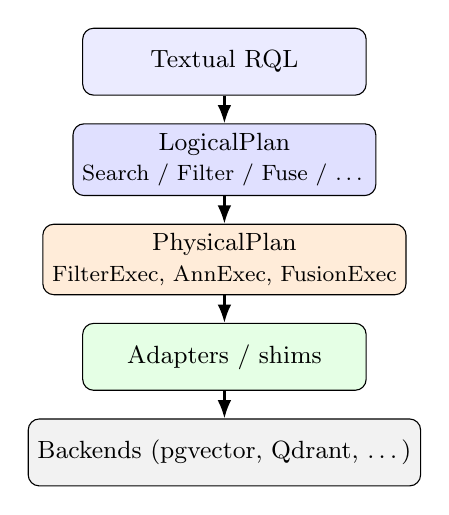
\begin{tikzpicture}[
  box/.style={draw, rounded corners, align=center, minimum width=3.6cm, minimum height=0.85cm, font=\small},
  arr/.style={-{Latex}, thick}
]
\node[box, fill=blue!8] (t) {Textual RQL};
\node[box, fill=blue!12, below=0.35cm of t] (l) {LogicalPlan\\{\footnotesize Search / Filter / Fuse / \ldots}};
\node[box, fill=orange!15, below=0.35cm of l] (p) {PhysicalPlan\\{\footnotesize FilterExec, AnnExec, FusionExec}};
\node[box, fill=green!10, below=0.35cm of p] (a) {Adapters / shims};
\node[box, fill=gray!10, below=0.35cm of a] (b) {Backends (pgvector, Qdrant, \ldots)};
\draw[arr] (t) -- (l);
\draw[arr] (l) -- (p);
\draw[arr] (p) -- (a);
\draw[arr] (a) -- (b);
\end{tikzpicture}

\caption{Hypothesized RQL compilation stack: text $\rightarrow$ logical plan $\rightarrow$ physical plan $\rightarrow$ adapters.}
\label{fig:stack}
\end{figure}

\section{Compilation and adapters}
\label{sec:compilation}

\noindent\textit{\hypothesis{} doctrine; Substrait/polystore inspiration is \provisional{}/\established{} as prior systems.}

\subsection{Layers}
\begin{enumerate}
  \item Parse textual RQL to \texttt{LogicalPlan}.
  \item Optimise to \texttt{PhysicalPlan} with capability negotiation.
  \item Emit backend calls through adapters (pgvector SQL, Qdrant query API, Pinecone, Neo4j, \ldots).
\end{enumerate}

\subsection{Capability negotiation}
Profiles declare required features (hybrid+RRF, graph hop, late interaction).
Missing capabilities yield either a safe rewrite, a shim CAST (e.g.\ client-side fuse---explicitly marked expensive/unsafe for ACL), or a hard error \hypothesis{}.

\subsection{Substrait adjacency}
Substrait~\citep{substrait} motivates a binary/portable plan encoding across engines.
RQL may eventually emit a retrieval-oriented dialect or embed custom extensions; this draft does not claim a finished Substrait specification \hypothesis{}.

\section{Applications to RAG patterns}
\label{sec:apps}

Patterns below map to example programs in the companion repo (\texttt{examples/*.rql}).

\begin{itemize}
  \item Dense + ACL metadata filter (reliability-first pushdown).
  \item Hybrid BM25+dense with RRF and optional cross-encoder rerank~\citep{cormack2009rrf}.
  \item Multi-query / HyDE-style rewrite as plan nodes (costed) \provisional{}.
  \item Parent expansion and bounded multi-hop graph retrieval \provisional{}.
  \item Late-interaction search with optional planner rewrite \provisional{}.
\end{itemize}

RQL's value is making these patterns \emph{comparable} under EXPLAIN and shared eval harnesses \hypothesis{}.

\section{Evaluation plan (no fabricated results)}
\label{sec:eval}

\noindent\textit{This section specifies \textbf{what we will measure}, not results we have not run.}

\subsection{Datasets (planned)}
\begin{itemize}
  \item Retrieval: BEIR/MS MARCO-style collections as available under license; synthetic metadata predicates for filter selectivity sweeps.
  \item Filtered-ANN microbenchmarks aligned with published FANNS setups (e.g.\ SIFT-scale vectors with attribute predicates), following protocols from prior work such as ACORN~\citep{patel2024acorn}---\textbf{re-run}, do not copy tables.
\end{itemize}
\textbf{HUMAN\_TODO:} dataset download, licenses, and digests --- see \texttt{experiments/HUMAN\_TODOS.md} and \texttt{experiments/protocols/02-datasets.md}.

\subsection{Metrics}
Recall@$k$, nDCG@$k$, latency p50/p95, throughput (QPS) where applicable, \textbf{plan stability} (same RQL $\rightarrow$ same logical plan hash), and ACL violation count (must be zero).

\subsection{Baselines}
\begin{enumerate}
  \item Hand-written SDK glue (LangChain/LlamaIndex-style scripts).
  \item Vendor filter+hybrid APIs directly.
  \item pgvector SQL hybrid patterns.
  \item Fixed \texttt{FILTER\_MODE} ablations vs \texttt{AUTO} (once implemented).
\end{enumerate}

\subsection{Ablation matrix (planned)}
Channels $\in\{$dense, bm25, both$\}$; fuse $\in\{$RRF, linear$\}$; filter mode $\in\{$PRE, POST, AUTO$\}$; rerank on/off; rewrite on/off.

\subsection{What exists today (agent-run)}
\begin{itemize}
  \item Planned-run printer: \texttt{experiments/harness/print\_planned\_runs.py} (emits \texttt{score=NOT\_RUN} only).
  \item Deterministic RRF unit test on fixed lists: \texttt{experiments/harness/test\_rrf\_fusion.py} $\rightarrow$ \texttt{experiments/results/rrf\_unit\_test.txt}.
  \item Deterministic weighted linear/CC fusion on fixed toy scores: \texttt{experiments/harness/test\_linear\_fusion.py} $\rightarrow$ \texttt{experiments/results/linear\_fusion/unit\_test.txt} (not an IR benchmark).
  \item Colab FANNS \emph{synthetic} microbench (T4 GPU, \texttt{faiss-gpu}~1.15.1; $N{=}50{,}000$, $d{=}128$, seed~$42$; selectivities $\{0.01,0.05,0.1,0.5\}$; modes PRE/POST): artifacts under \texttt{experiments/results/fanns/colab\_synth\_20260916\_233628/} (journal~0029; notebook URL in \texttt{experiments/colab/LINKS.md}).
\end{itemize}

\paragraph{Honest label for the Colab synthetic run.}
This run is \textbf{plumbing + qualitative PRE vs POST latency/QPS shape on synthetic data} only.
It is \textbf{not} P0: SIFT1M (or another licensed large vector set) with ground-truth $k$NN was \textbf{not} run.
Recall@$10{=}1.0$ on this easy synthetic predicate setup is \textbf{not} a citation-ready ANN quality claim --- do not treat the numbers as paper results or as ACORN/FANNS table reproductions.
See Appendix~\ref{sec:repro} for the artifact checklist.

\textbf{No end-to-end RAG, BEIR, or human-judgment metrics are claimed. No licensed large-set FANNS P0 is claimed.}

\subsection{What requires a human (Vijay)}
GPU/CPU FANNS microbench, production/docker vector DB smokes, paid APIs, large datasets, and relevance judgments are listed as \textbf{HUMAN\_TODO} items with exact protocols and expected in-repo artifact paths in \texttt{experiments/HUMAN\_TODOS.md}.
Those results should be pushed to this same GitHub repository when available.

\section{Threats to validity}
\label{sec:threats}

\begin{itemize}
  \item \textbf{Literature coverage:} only ACORN has completed multimodal Pass~1--5 in-repo; other citations remain \provisional{}.
  \item \textbf{ANN nondeterminism:} recall is implementation-dependent; portable IR cannot claim bit-identical results.
  \item \textbf{Adapter impedance:} not all backends expose subgraph or hybrid fusion; shims may hide costs.
  \item \textbf{Optimism bias:} algebra elegance does not guarantee planner quality without measured cost models.
\end{itemize}

\section{Conclusion}
\label{sec:conclusion}

We framed RQL as a \textbf{portable retrieval-plan IR} for RAG---algebra plus physical planning under recall/latency/ACL---rather than as cosmetic SQL for vectors \hypothesis{}.
ACORN's multimodal re-read \established{} the need to treat filter strategy as a first-class physical decision~\citep{patel2024acorn}.
The immediate path is: finish Pass~1--5 on VBASE and Filtered-DiskANN, freeze a LogicalPlan schema, implement two adapters, and execute the evaluation plan with published artifacts---without shortcutting integrity.

\appendix
\section{Reproducibility checklist}
\label{sec:repro}

\begin{enumerate}
  \item Scripts and configs under \texttt{experiments/} with pinned dependency files when benchmarks are added.
  \item Dataset license notes and download digests (\textbf{HUMAN\_TODO}: \texttt{experiments/protocols/02-datasets.md}).
  \item Seeded RNGs where stochasticity exists; report ANN library versions in \texttt{ENV.txt}.
  \item Store logical/physical plan JSON beside metrics (no orphaned scores).
  \item Separate AUTHOR\_CLAIM citations from REPRODUCED runs in result tables.
  \item Research notes: journal + OKF-shaped bundles for paper reads.
  \item Hand-off list for compute/credentials beyond the agent sandbox: \texttt{experiments/HUMAN\_TODOS.md}.
\end{enumerate}

\subsection{Colab synthetic FANNS smoke (in-repo, not P0)}
\label{sec:repro-colab-synth}
Run id \texttt{colab\_synth\_20260916\_233628} (Europe/Dublin wall clock aligned with journal~0029):
\begin{itemize}
  \item Path: \texttt{experiments/results/fanns/colab\_synth\_20260916\_233628/} (\texttt{metrics.json}, \texttt{ENV.txt}, \texttt{plans/}).
  \item Colab notebook URL registry: \texttt{experiments/colab/LINKS.md}.
  \item Backend: \texttt{faiss-gpu}~1.15.1 on T4; synthetic Gaussian vectors only.
  \item \textbf{What it supports:} harness wiring and a qualitative PRE$\ll$POST latency/QPS shape on this synthetic setup.
  \item \textbf{What it does not support:} P0 claims, SIFT1M completion, or citation-ready filtered-ANN recall tables.
\end{itemize}


\bibliographystyle{plainnat}
\bibliography{references}

\end{document}
